\chapter{Results}
\label{results}

In this chapter we present the results of our simulation. In the first section we will present the default and individualized lifecycle investment strategies, the former being provided by real retirement funds and the latter being solved by Merton and Munk. We will plug in the heterogeneous parameters, described in detail in the previous chapter. In the next section, we will calculate the resulting financial capital flows and compare their welfare effects using their expected utilities, as mentioned in Chapter 3. 

\section{Investment strategies}
\subsection{Default lifecyccles}
As was discussed in the previous chapter, our individual decides between investing in risky (stocks) or risk-free (bonds) assets. The default allocations for share of risky asset are given by:

\begin{itemize}
	\item $100-t$, for all $t$
	\item $\begin{cases} 100\%, & t<40\\(200-2.5t)\%, & t\in[40,57]\end{cases}$
	\item $63\%$, for all $t$
	\item $30\%$, for all $t$
\end{itemize}

where the latter two are Markowitz's solution and Anadolu Hayat's moderate investment option respectively. Since we are only interested in age span between 28 and 57, Figure 5.1 shows the risky asset share $\pi_t$ only for that interval. 

\begin{figure}[h]
	\centering
	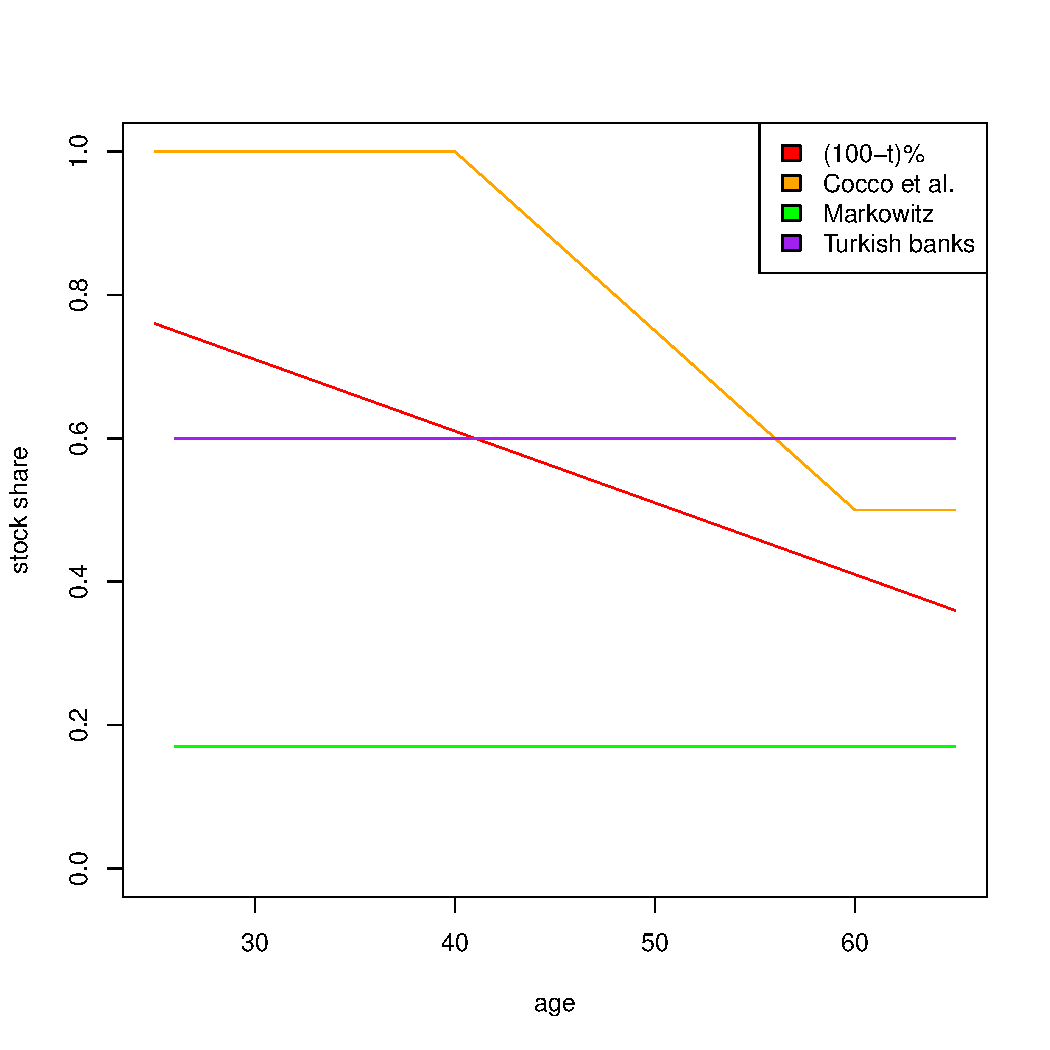
\includegraphics[scale=0.6]{figs/defaults.pdf}
	\caption{Default portfolio allocations of stock investments}
\end{figure}


\subsection{Individualized lifecycles}

To derive individualized lifecycle strategies, we used Merton's (1971) and Munk's (2016) optimal portfolio allocation formulas mentioned in chapters 2 and 3. Since these formulas depended on intratemporal amounts of capital, we have constructed three human capital series corresponding to flat, moderate and steep wage growth curves mentioned in the previous chapter. Figure 5.2 illustrates the risky asset shares given by Merton and Munk without housing for various levels of labor income growth and risk aversion. The figure shows that the steeper the wage growth curves get or the lower their risk aversion is, the more aggressive investors are. However, as a whole, they follow the similar pattern. The figure also shows that for small correlations between labor income and stock prices, Munk's solution converges to Merton's solution, as was shown in Chapter 3.

\begin{figure}
	\centering
    \begin{subfigure}{0.45\textwidth}
		\centering
		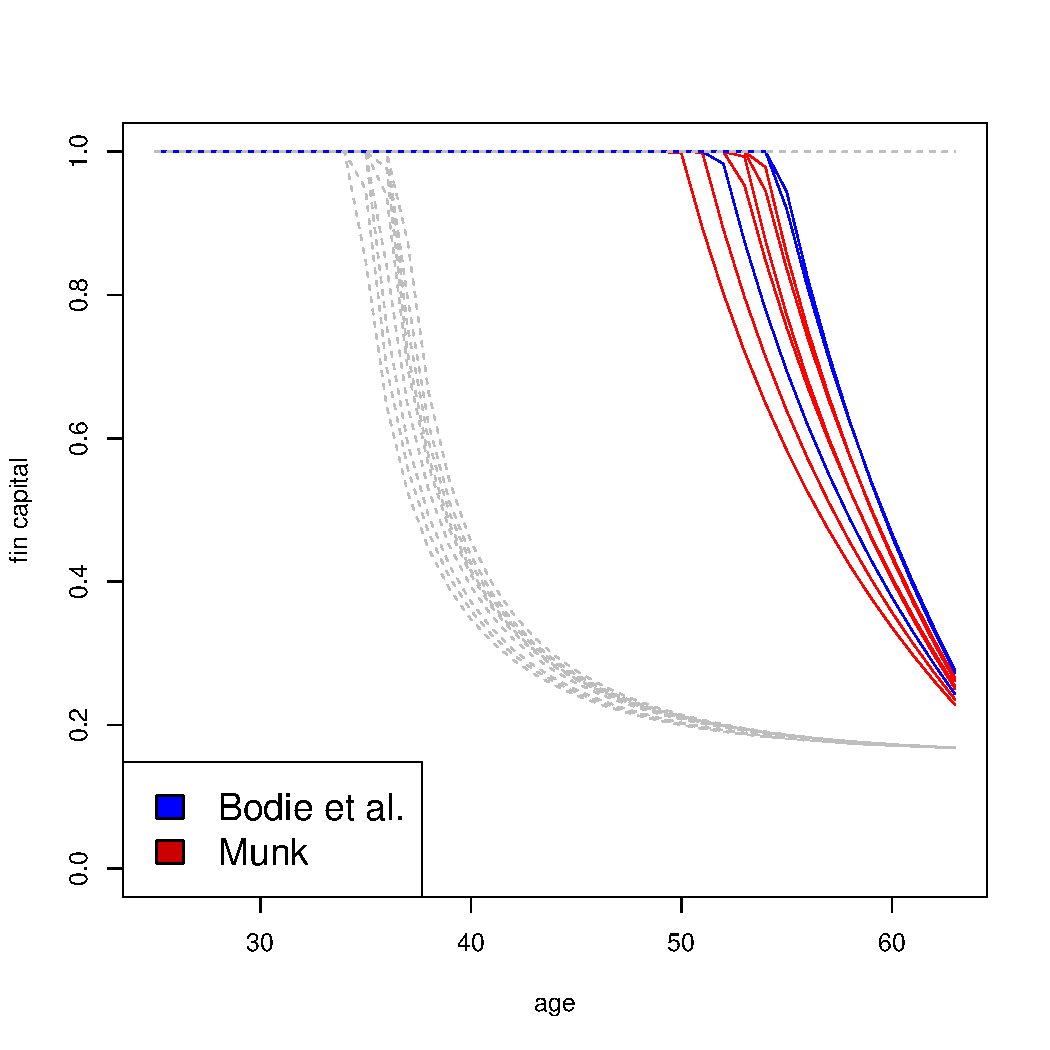
\includegraphics[scale=0.4]{figs/individuals15.pdf}
		\caption{$\gamma = 1.5$}
	\end{subfigure}
	\hfill
    \begin{subfigure}{0.45\textwidth}
		\centering
		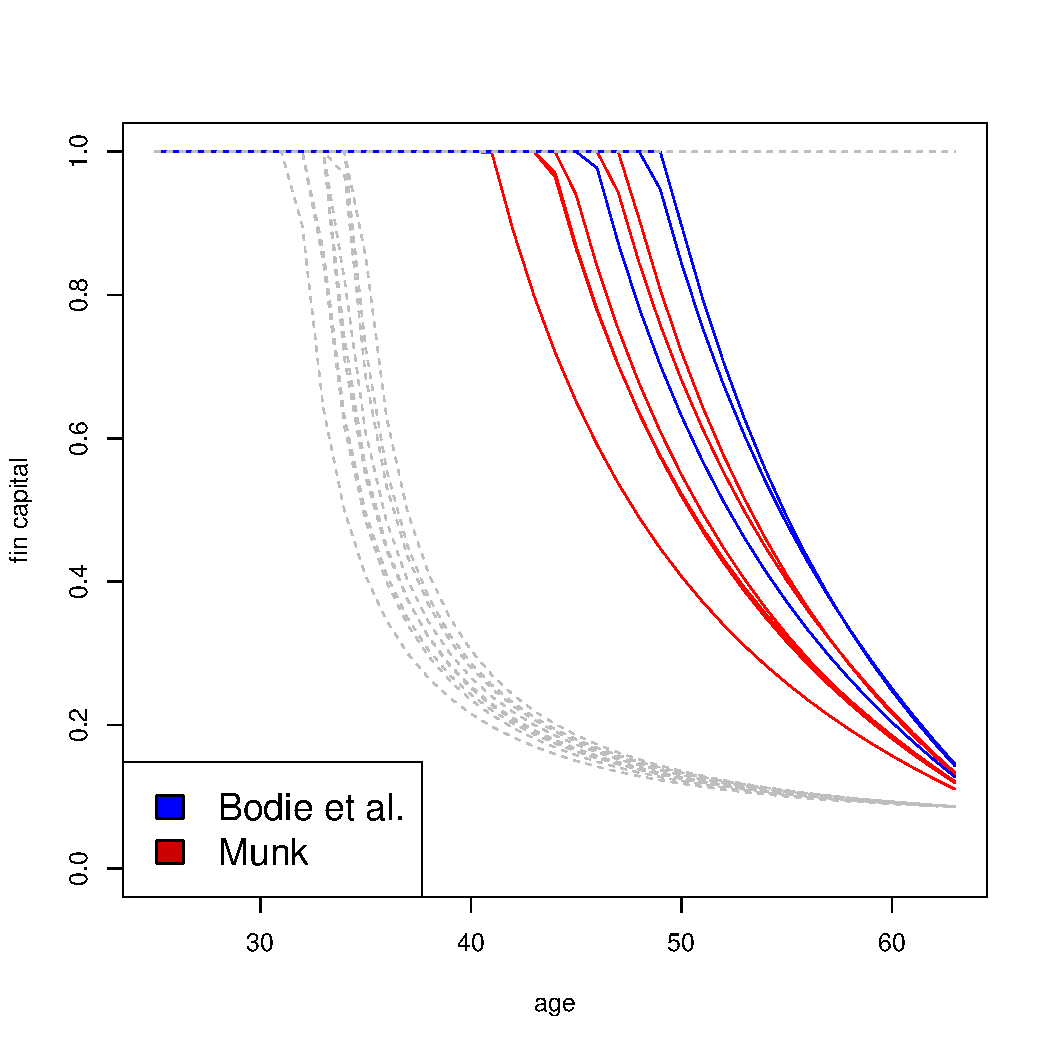
\includegraphics[scale=0.4]{figs/individuals3.pdf}
		\caption{$\gamma = 3$}
	\end{subfigure}
	\hfill
    \begin{subfigure}{0.45\textwidth}
		\centering
		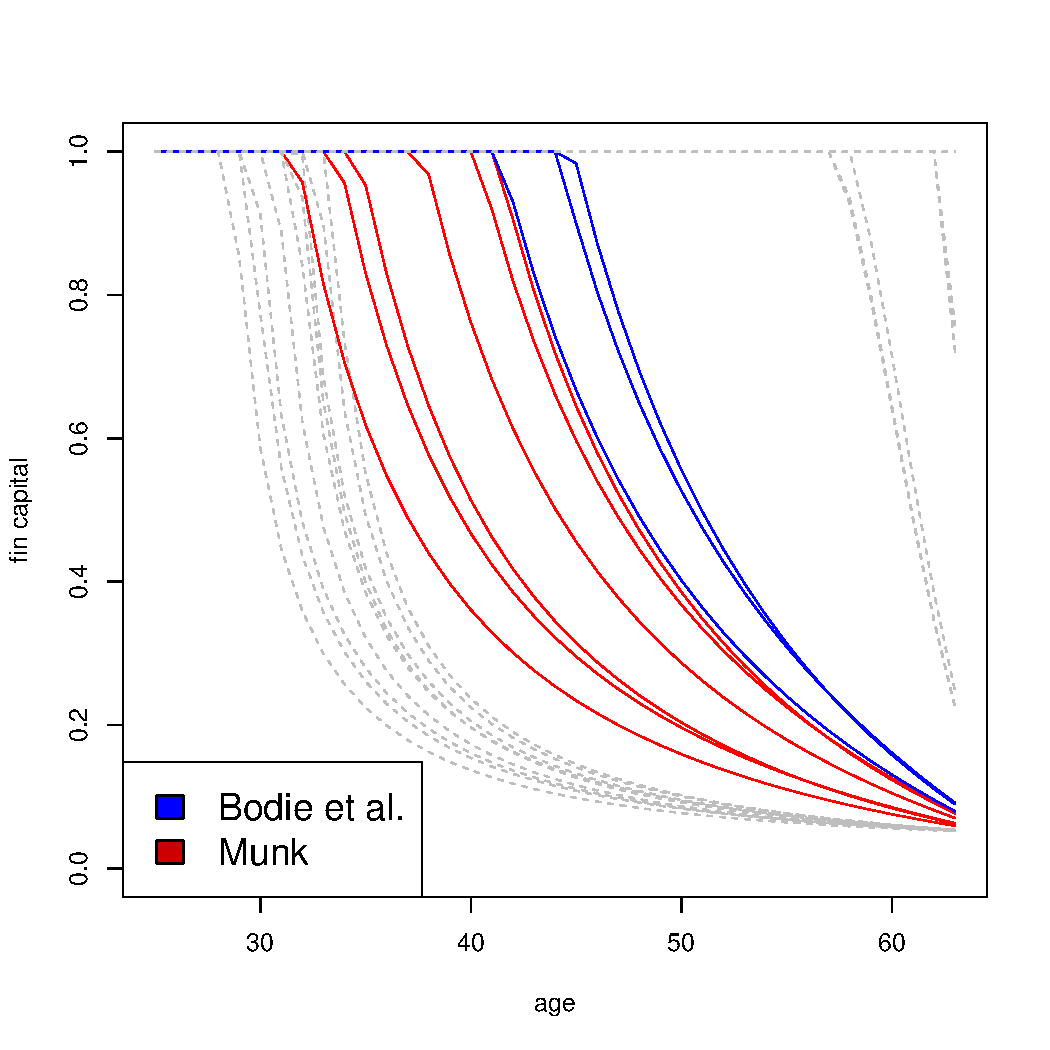
\includegraphics[scale=0.4]{figs/individuals5.pdf}
		\caption{$\gamma = 5$}
	\end{subfigure}
	\hfill
    \begin{subfigure}{0.45\textwidth}
		\centering
		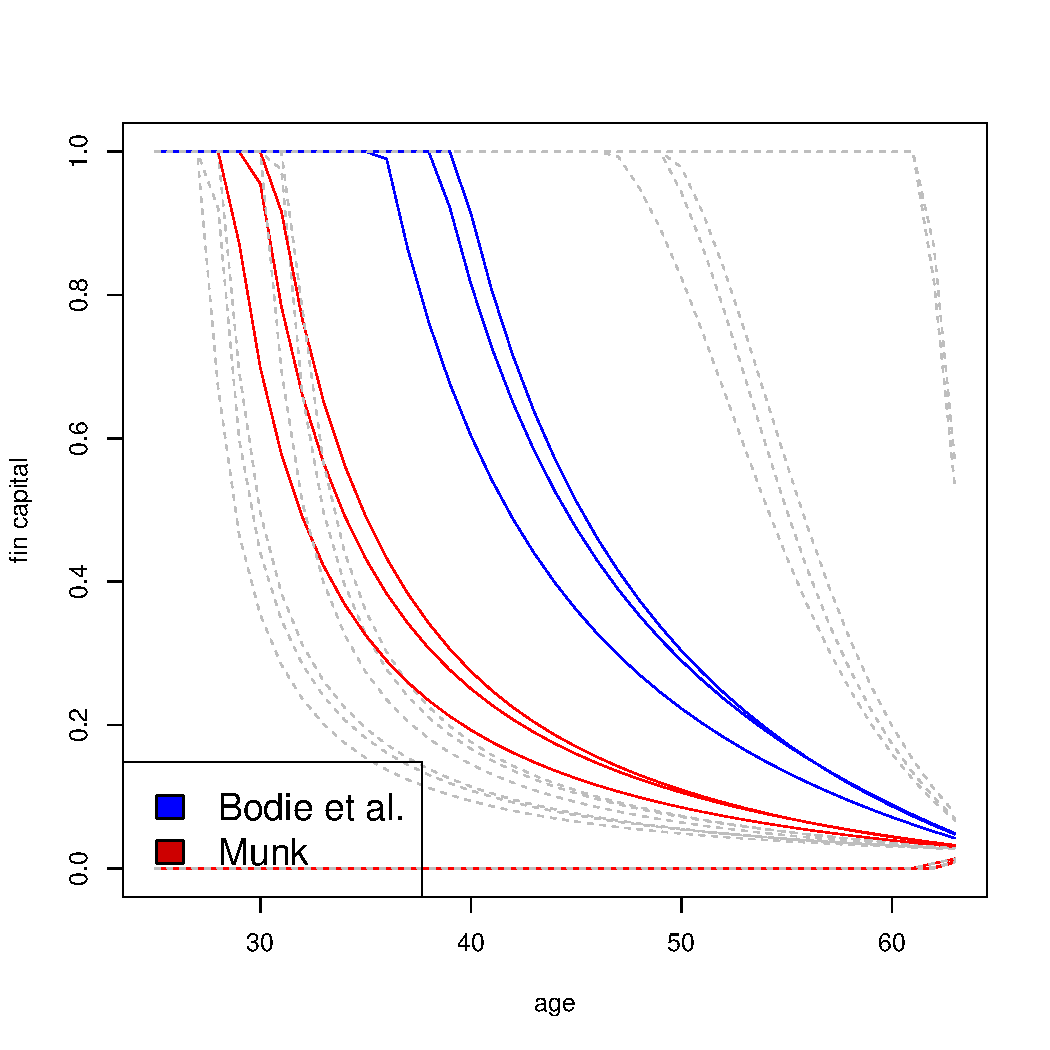
\includegraphics[scale=0.4]{figs/individuals10.pdf}
		\caption{$\gamma = 10$}
	\end{subfigure}
	\caption{Merton and Munk's solution without housing for different wage growth and risk aversion levels}
\end{figure}

\paragraph{}Figure 5.3 illustrates the stock and housing asset shares determined by Munk with housing for flat, moderate and steep labor income curves and low, moderate and high stock-labor income correlations for different levels of risk aversion, to capture heterogeneity, as mentioned in the previous chapter. The figure confirms that steeper labor income curves result in larger share of stocks in portfolio and less of bonds. Around age of 45, the sum of optimal stock and housing investments falls below $1$ and optimal bond investment becomes positive. Also, the higher the risk aversion, the less the individuals want to invest in both housing and stocks --- for $\gamma=10$, the optimal Munk solutions are negative or add up to less than $1$, meaning that they should sell all stocks and housing to invest in risk-free long term bonds. In our analysis we do not allow for negative investing, since this is not a primary focus of our thesis.  



\paragraph{}Full tables with actual solutions are available in Tables E.1 and E.2 of Appendix E for models without housing and in Table E.3 for a model with housing. 


\section{Welfare comparison}

In order to compare welfare we use CRRA expected utility function, mentioned in Chapter 3. The probabilities of survival are taken from TUIK as mentioned in the previous chapter. The consumption is calculated in numbers of consumption baskets which cost exactly $1$ CPI --- consumer price index at that period, which is increasing with inflation rate annually, and is equal to $100$ at retirement age $57$. The wealth for which consumption baskets are purchased is a total accumulated wealth, including stock returns, bond returns and housing returns, annuitized according to the formula described in Chapter 3. Discount rate is $0.89$, as mentioned in the previous chapter. We compare expected utilities for different levels of risk aversion.

\begin{figure}[H]
	\centering
    \begin{subfigure}{0.45\textwidth}
		\centering
		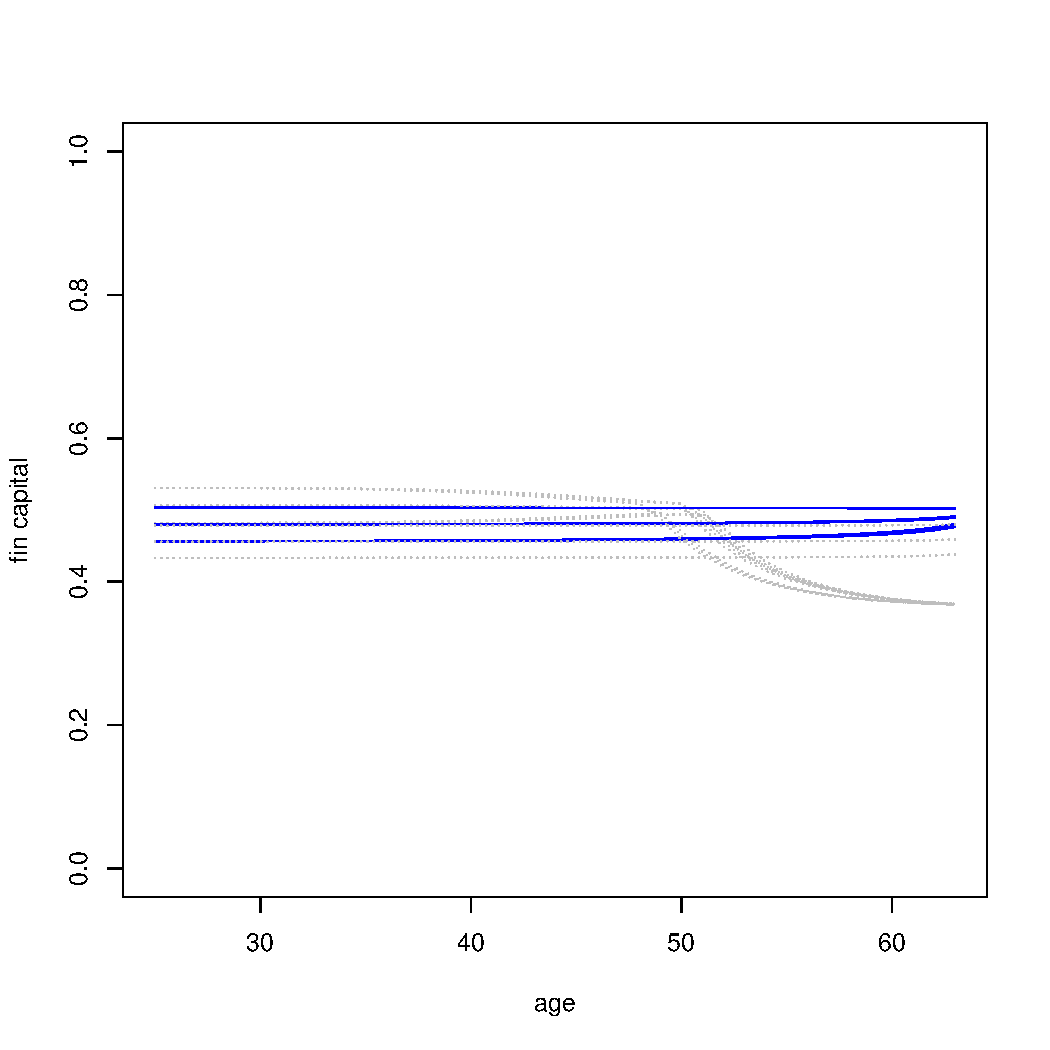
\includegraphics[scale=0.4]{figs/smunkhouse15.pdf}
		\caption{Stocks for $\gamma = 1.5$}
	\end{subfigure}
	\hfill
    \begin{subfigure}{0.45\textwidth}
		\centering
		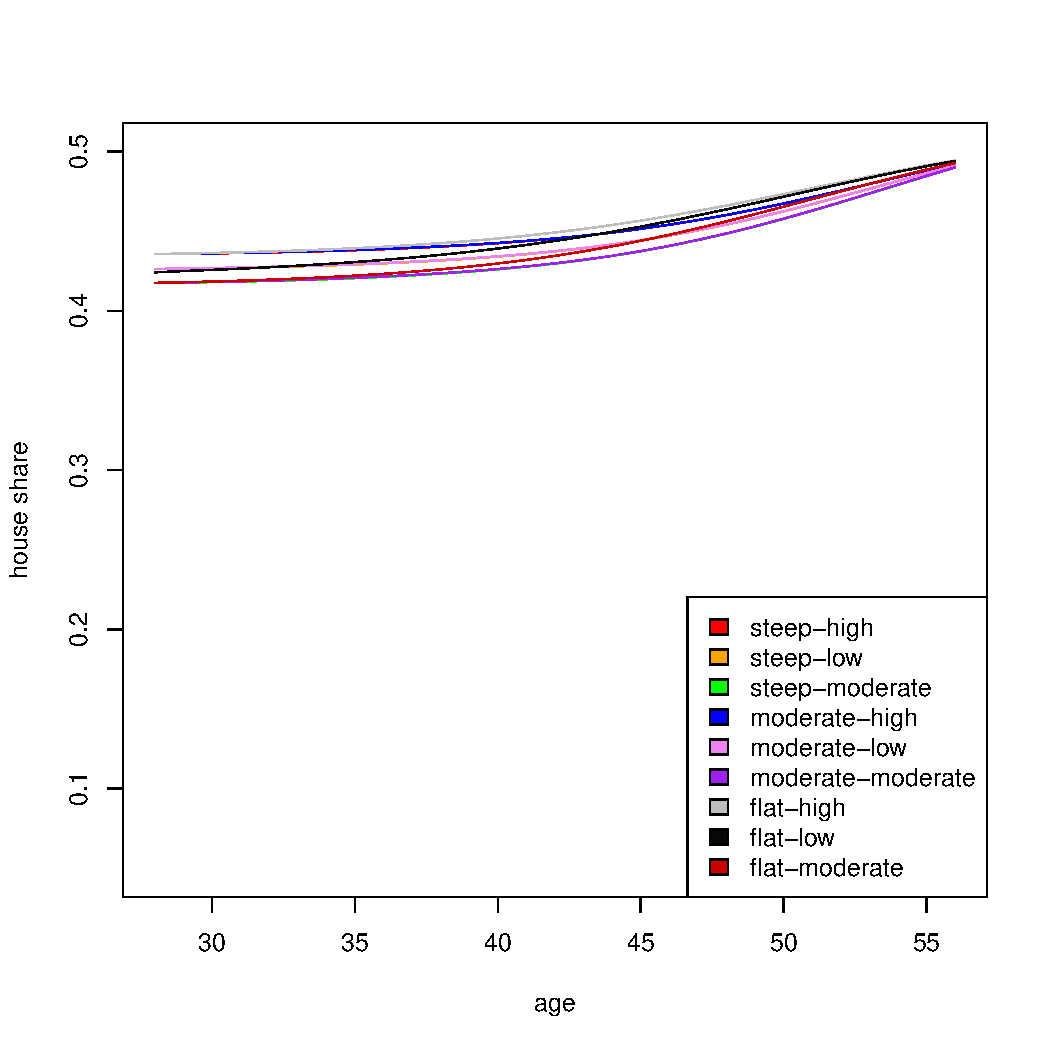
\includegraphics[scale=0.4]{figs/hmunkhouse15.pdf}
		\caption{Housing for $\gamma = 1.5$}
	\end{subfigure}
	\hfill
    \begin{subfigure}{0.45\textwidth}
		\centering
		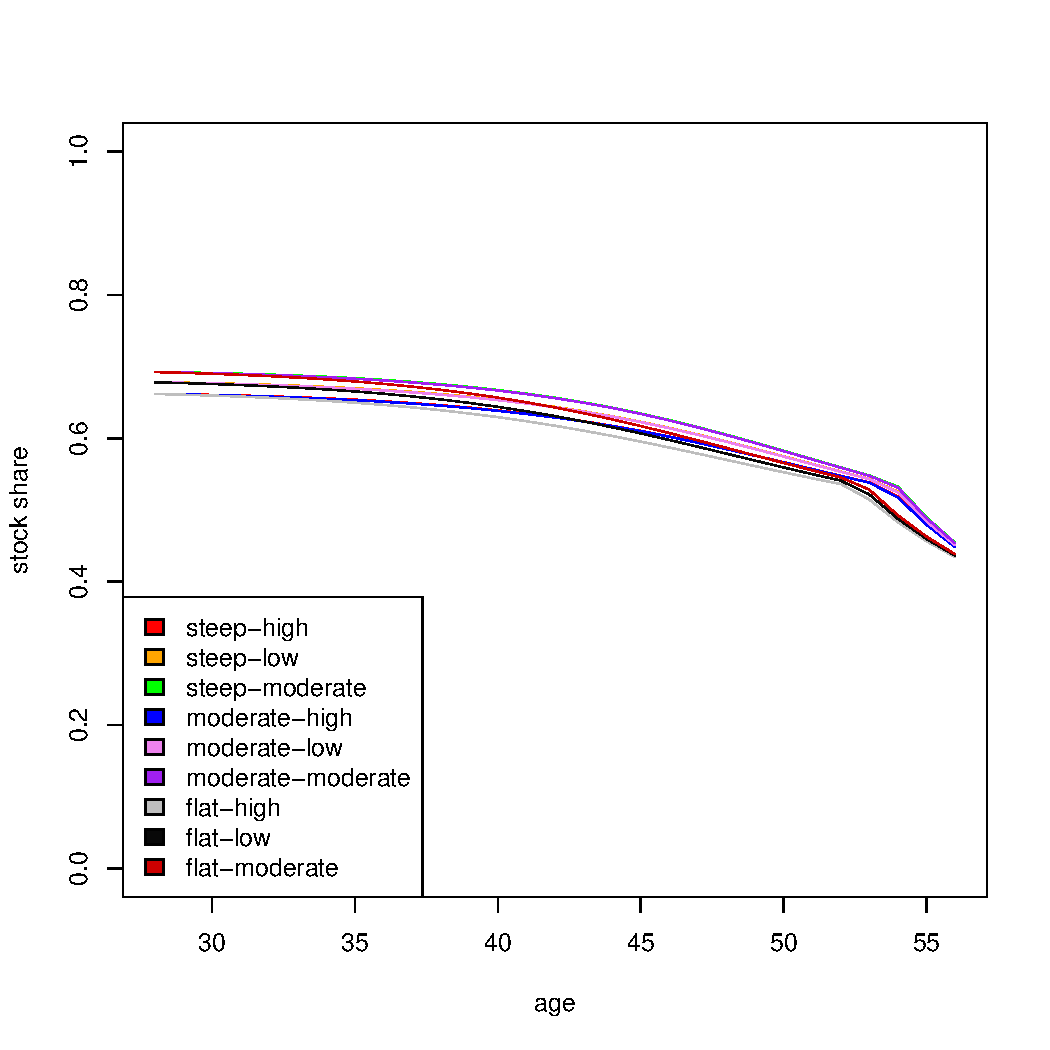
\includegraphics[scale=0.4]{figs/smunkhouse3.pdf}
		\caption{Stocks for $\gamma = 3$}
	\end{subfigure}
	\hfill
    \begin{subfigure}{0.45\textwidth}
		\centering
		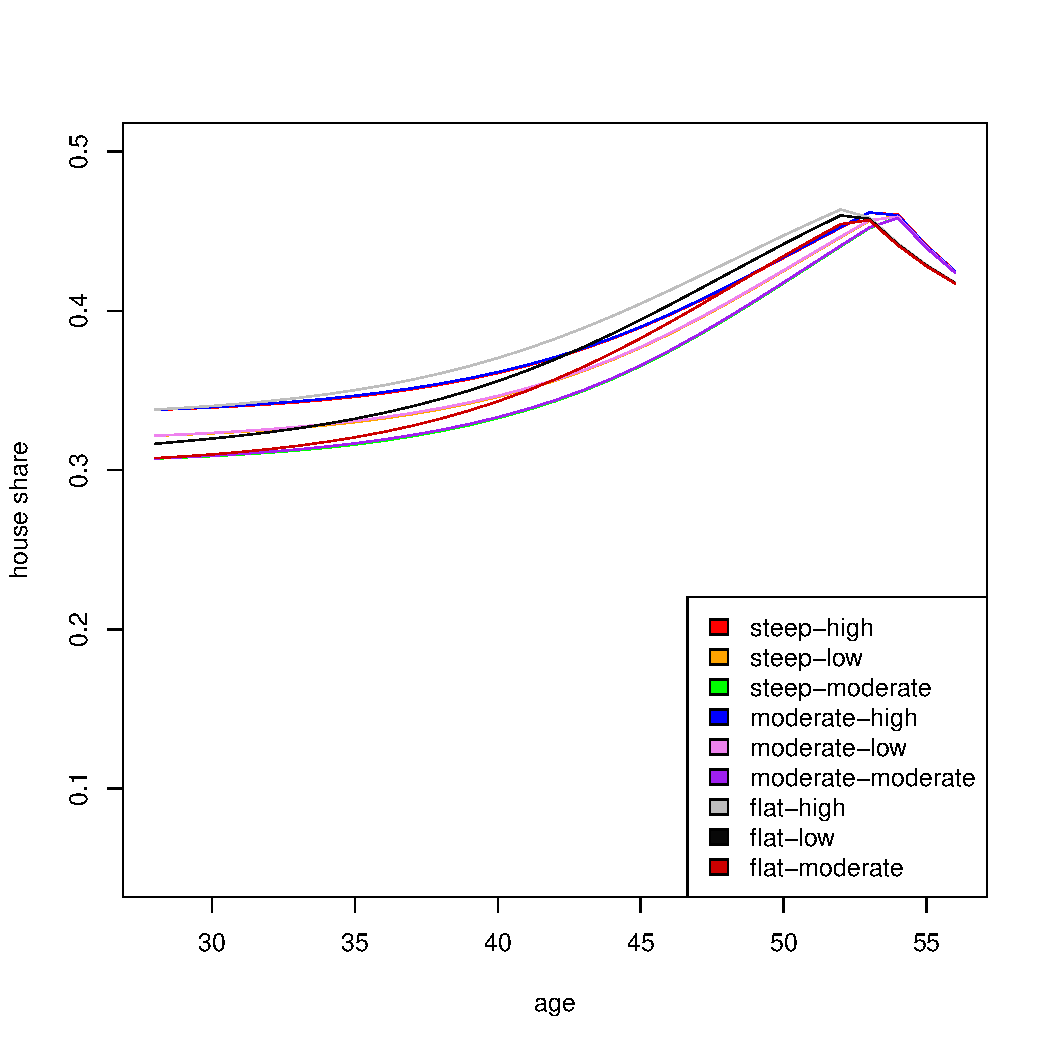
\includegraphics[scale=0.4]{figs/hmunkhouse3.pdf}
		\caption{Housing for $\gamma = 3$}
	\end{subfigure}
	\hfill
    \begin{subfigure}{0.45\textwidth}
		\centering
		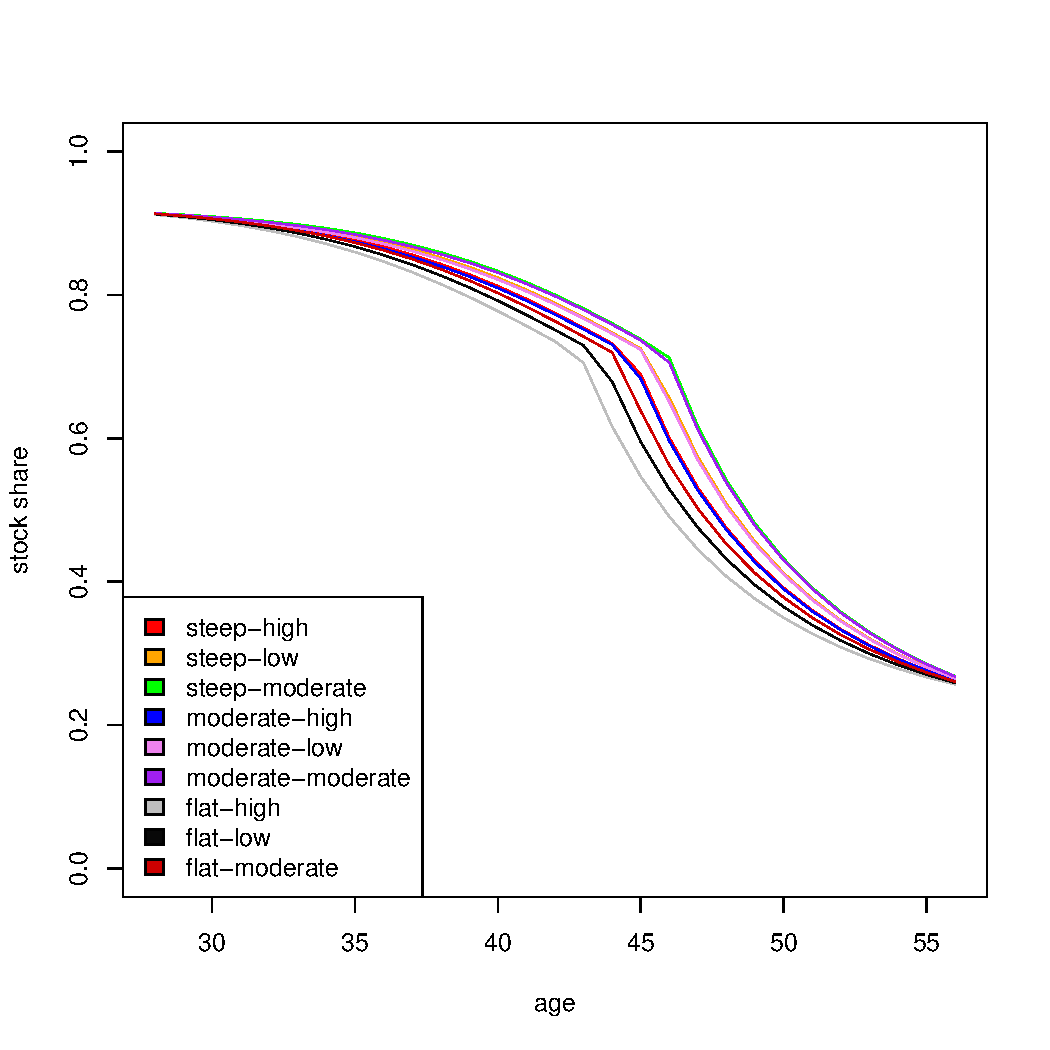
\includegraphics[scale=0.4]{figs/smunkhouse5.pdf}
		\caption{Stocks for $\gamma = 5$}
	\end{subfigure}
	\hfill
    \begin{subfigure}{0.45\textwidth}
		\centering
		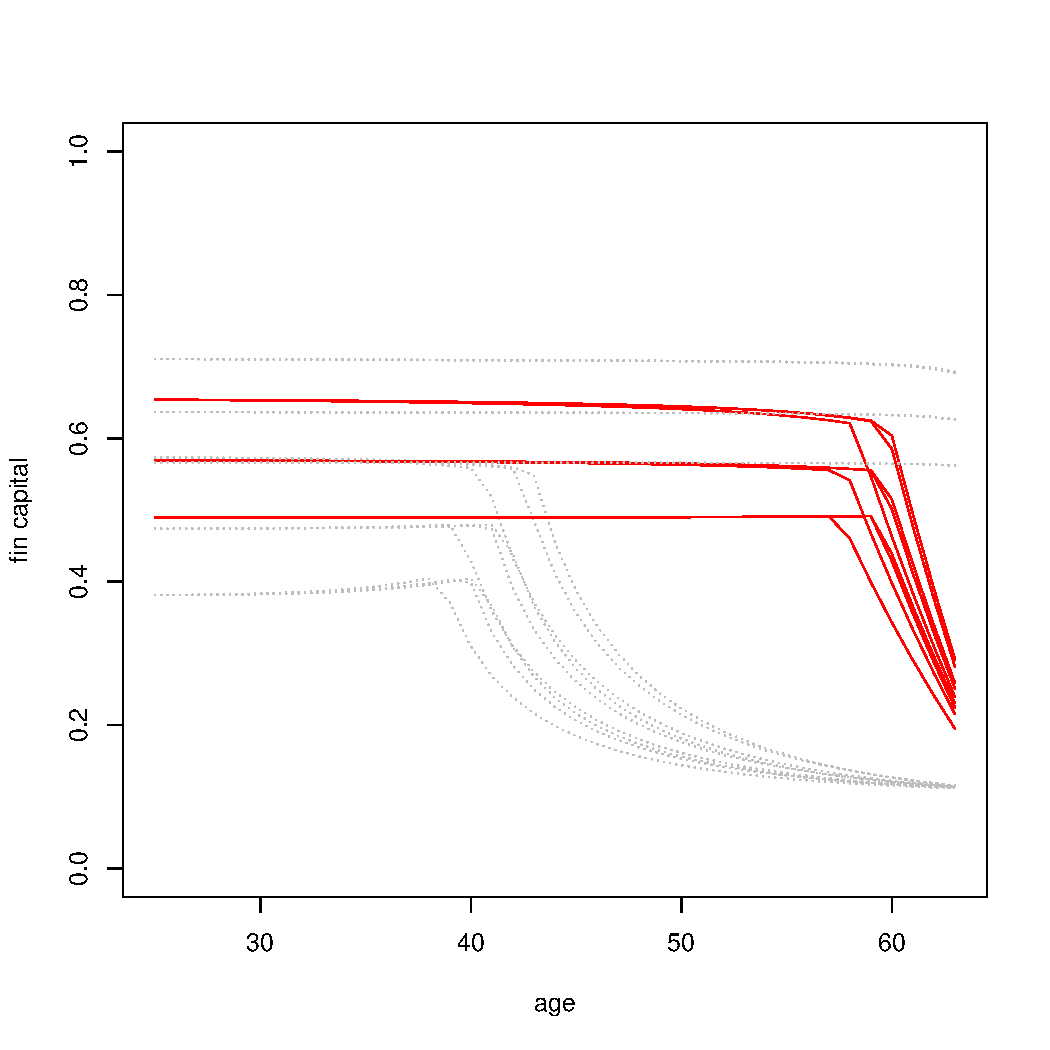
\includegraphics[scale=0.4]{figs/hmunkhouse5.pdf}
		\caption{Housing for $\gamma = 5$}
	\end{subfigure}
\end{figure}
\begin{figure}[H]\ContinuedFloat
    \begin{subfigure}{0.45\textwidth}
		\centering
		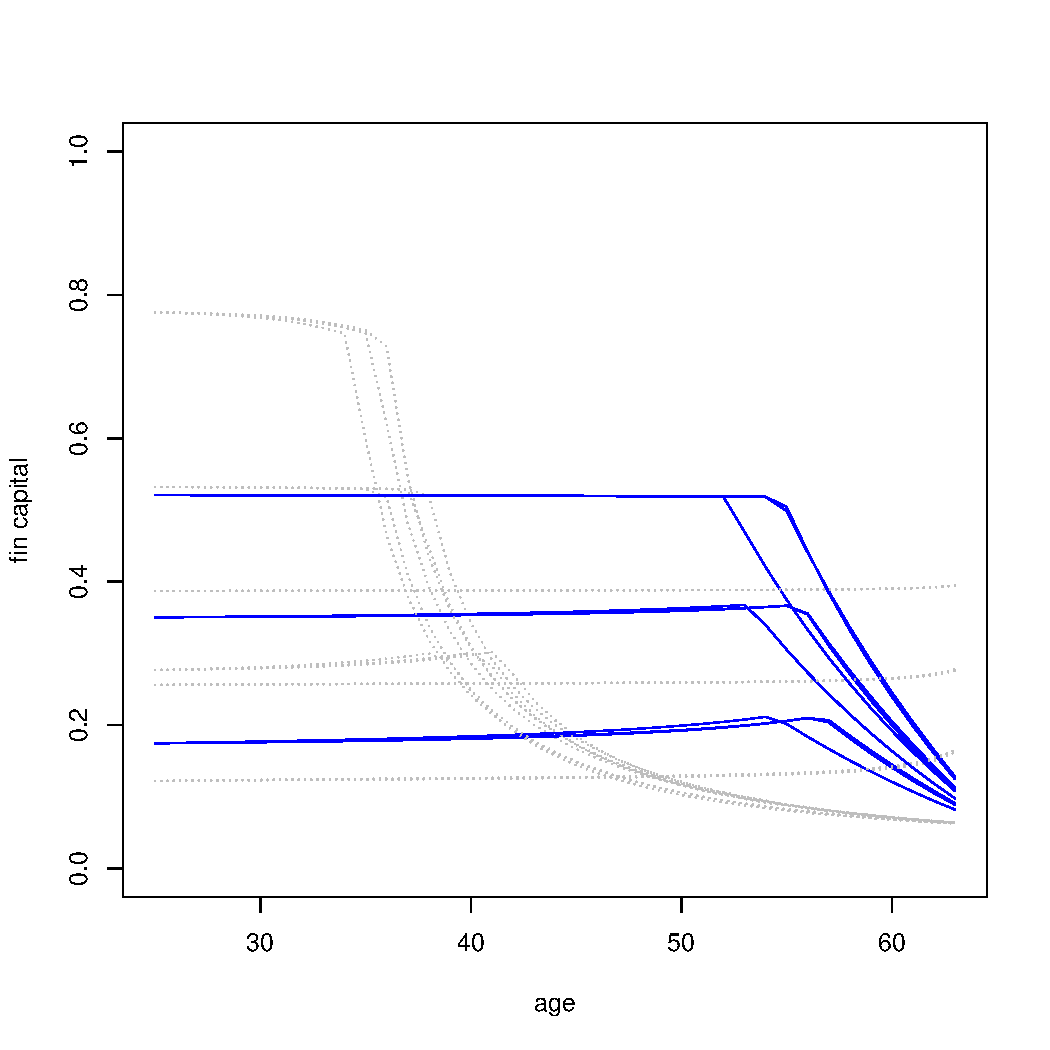
\includegraphics[scale=0.4]{figs/smunkhouse10.pdf}
		\caption{Stocks for $\gamma = 10$}
	\end{subfigure}
	\hfill
    \begin{subfigure}{0.45\textwidth}
		\centering
		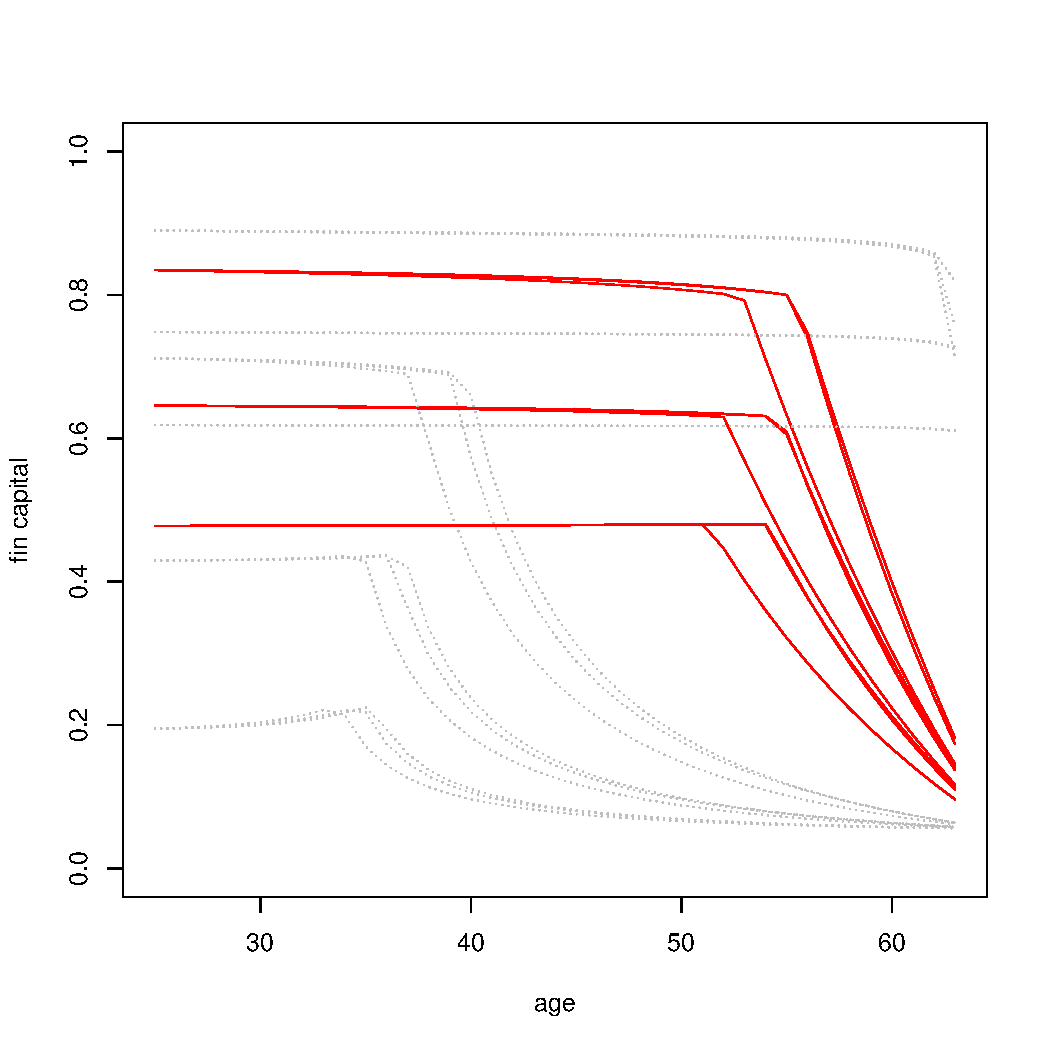
\includegraphics[scale=0.4]{figs/hmunkhouse10.pdf}
		\caption{Housing for $\gamma = 10$}
	\end{subfigure}
	\caption{Munk's stock and housing shares for different wage growth, stock-wage correlation and risk aversion levels}
\end{figure}

\subsection{Early results}

After a lifetime of investing in the above portfolios, the household accumulates different levels of wealth, summarized in Table 5.1. Since the consumption preferences are monotonic, we can make early conclusions even without calculating expected utilities --- the higher the accumulated wealth, the better: 

\begin{itemize}
\item Naively considering lifecycles does not guarantee the better investment. So, in our case, $(100-age)\%$ is worse than fixed Markowitz.
\item Different stock-wage correlations don't make much difference in the outcome without housing, and make considerable difference in models with housing
\item Stock-wage correlations are negatively correlated with total wealth
\item Both too low and too high risk aversion results in less accumulated capital than moderate risk aversion for models with housing and only too high risk aversion --- for models without housing (because of monotonicity).\\
\item Default options are better for people with flat wage growth rate and worse for people with moderate or steep wage curves
\end{itemize}

\subsection{Annuitization}
To formalize the observations made in the previous section, we will construct annuities and plug them into expected utility functions. As described in detail in Chapter 3, we define annuities by dividing the total wealth before retirement by the discount factor $1 + \sum^{100}_{t=58}\frac{p_t}{1+r_f}$. Using survival probabilities, obtained from TUIK, and risk-free rate of return, described in the previous chapter, we calculate the discount factor as $205.29$. The annuities are obtained by dividing all the values in the Table 5.1 by $205.29$. The resulting values are presented in Table 5.2. 


\subsection{Consumption during retirement}
We model that the individuals spend their annuity returns to consume baskets which cost $100$ TL during the year, when our agent is 58 years old, and increase by inflation rate $\pi = 8.4\%$. Thus, every period $t>57$ our agent consumes $\frac{annuity}{100\cdot\left(1.084\right)^{t-58}}$. We do not provide the separate table with the value streams, as they will be implicitly included in utility values.


\subsection{Expected utilities}
Finally, we will plug the consumption streams, calculated in the previous section, into the constant relative risk-aversion expected utility functions to compare the welfare effects. The resulting expected utility values are presented in Table 5.3.


\newgeometry{top=2cm,bottom=2cm}
\begin{table}%TABLE 5.1
	\centering
	\caption{Total Accumulated Wealth by Investment Option}
	\begin{tabular}[c]{lrrrr}
		\hline
		Option&$\gamma=5$ (default) & $\gamma=1.5$ & $\gamma=3$ & $\gamma=10$\\
		\hline
		\multicolumn{5}{c}{Defaults}\\
Anadolu Hayat (riskless)&614,195 TL&614,195 TL&614,195 TL&614,195 TL\\
$(100-age)\%$&1,160,977 TL&1,160,977 TL&1,160,977 TL&1,160,977 TL\\
Cocco et al.&1,599,852 TL&1,599,852 TL&1,599,852 TL&1,599,852 TL\\
Markowitz&1,300,187 TL&1,300,187 TL&1,300,187 TL&1,300,187 TL\\
\multicolumn{5}{c}{}\\
\multicolumn{5}{c}{Individualized (no housing)}\\
Merton (steep)&3,812,053 TL&4,212,735 TL&3,104,746 TL&2,920,892 TL\\
Merton (moderate)&1,629,904 TL&1,813,821 TL&1,447,951 TL&1,248,330 TL\\
Merton (flat)&543,602 TL&612,548 TL&639,866 TL&398,235 TL\\
Munk (steep-lo)&3,547,442 TL&4,168,823 TL&3,829,218 TL&2,085,883 TL\\
Munk (steep-mod)&3,543,435 TL&4,164,850 TL&3,825,221 TL&2,081,872 TL\\
Munk (steep-hi)&3,539,425 TL&4,160,872 TL&3,821,219 TL&2,077,854 TL\\
Munk (moderate-lo)&1,513,198 TL&1,794,772 TL&1,689,491 TL&868,955 TL\\
Munk (moderate-mod)&1,511,527 TL&1,793,113 TL&1,687,822 TL&867,281 TL\\
Munk (moderate-hi)&1,509,853 TL&1,791,452 TL&1,686,152 TL&865,604 TL\\
Munk (flat-lo)&508,757 TL&606,410 TL&657,762 TL&262,161 TL\\
Munk (flat-mod)&508,371 TL&606,025 TL&657,376 TL&261,774 TL\\
Munk (flat-hi)&507,984 TL&605,640 TL&656,990 TL&261,386 TL\\
\multicolumn{5}{c}{}\\
\multicolumn{5}{c}{Individualized (no housing)}\\
Munk (steep-lo)&8,937,159 TL&3,087,377 TL&4,718,332 TL&3,920,863 TL\\
Munk (steep-mod)&7,645,621 TL&2,966,467 TL&4,371,031 TL&2,900,022 TL\\
Munk (steep-hi)&6,353,327 TL&2,846,577 TL&4,017,054 TL&1,872,799 TL\\
Munk (moderate-lo)&3,652,223 TL&1,304,014 TL&1,998,234 TL&1,605,470 TL\\
Munk (moderate-mod)&3,125,930 TL&1,252,432 TL&1,850,278 TL&1,189,240 TL\\
Munk (moderate-hi)&2,599,301 TL&1,201,297 TL&1,700,235 TL&770,295 TL\\
Munk (flat-lo)&1,026,845 TL&430,353 TL&614,929 TL&455,296 TL\\
Munk (flat-mod)&881,934 TL&435,168 TL&598,789 TL&341,199 TL\\
Munk (flat-hi)&736,896 TL&397,829 TL&527,533 TL&226,188 TL\\
		\hline
	\end{tabular}
\end{table}
\resetgeometry


\newgeometry{top=2cm,bottom=2cm}
\begin{table}%TABLE 5.2
	\centering
	\caption{Annual Pensions by Investment Option}
	\begin{tabular}[c]{lrrrr}
		\hline
		Option&$\gamma=5$ (default) & $\gamma=1.5$ & $\gamma=3$ & $\gamma=10$\\
		\hline
		\multicolumn{5}{c}{Defaults}\\
Anadolu Hayat (riskless) TL&2,992 TL&2,992 TL&2,992 TL&2,992 TL\\
$(100-age)\%$ TL&5,655 TL&5,655 TL&5,655 TL&5,655 TL\\
Cocco et al. TL&7,793 TL&7,793 TL&7,793 TL&7,793 TL\\
Markowitz TL&6,333 TL&6,333 TL&6,333 TL&6,333 TL\\
\multicolumn{5}{c}{}\\
\multicolumn{5}{c}{Individualized (no housing)}\\
Merton (steep) TL&18,569 TL&20,521 TL&15,124 TL&14,228 TL\\
Merton (moderate) TL&7,940 TL&8,835 TL&7,053 TL&6,081 TL\\
Merton (flat) TL&2,648 TL&2,984 TL&3,117 TL&1,940 TL\\
Munk (steep-lo) TL&17,280 TL&20,307 TL&18,653 TL&10,161 TL\\
Munk (steep-mod) TL&17,261 TL&20,288 TL&18,633 TL&10,141 TL\\
Munk (steep-hi) TL&17,241 TL&20,268 TL&18,614 TL&10,122 TL\\
Munk (moderate-lo) TL&7,371 TL&8,743 TL&8,230 TL&4,233 TL\\
Munk (moderate-mod) TL&7,363 TL&8,735 TL&8,222 TL&4,225 TL\\
Munk (moderate-hi) TL&7,355 TL&8,726 TL&8,214 TL&4,216 TL\\
Munk (flat-lo) TL&2,478 TL&2,954 TL&3,204 TL&1,277 TL\\
Munk (flat-mod) TL&2,476 TL&2,952 TL&3,202 TL&1,275 TL\\
Munk (flat-hi) TL&2,474 TL&2,950 TL&3,200 TL&1,273 TL\\
\multicolumn{5}{c}{}\\
\multicolumn{5}{c}{Individualized (housing)}\\
Munk (steep-lo) TL&43,534 TL&15,039 TL&22,984 TL&19,099 TL\\
Munk (steep-mod) TL&37,243 TL&14,450 TL&21,292 TL&14,126 TL\\
Munk (steep-hi) TL&30,948 TL&13,866 TL&19,568 TL&9,123 TL\\
Munk (moderate-lo) TL&17,791 TL&6,352 TL&9,734 TL&7,820 TL\\
Munk (moderate-mod) TL&15,227 TL&6,101 TL&9,013 TL&5,793 TL\\
Munk (moderate-hi) TL&12,662 TL&5,852 TL&8,282 TL&3,752 TL\\
Munk (flat-lo) TL&5,002 TL&2,096 TL&2,995 TL&2,218 TL\\
Munk (flat-mod) TL&4,296 TL&2,120 TL&2,917 TL&1,662 TL\\
Munk (flat-hi) TL&3,590 TL&1,938 TL&2,570 TL&1,102 TL\\

		\hline
	\end{tabular}
\end{table}
\resetgeometry

\subsection{Conclusions}
Now, we can observe the final resutls:

\begin{itemize}

\item Naive lifecycle investment portfolios, such as $(100-age)\%$ don't overperform fixed-ratio Markowitz, because they don't take the risk aversion into consideration.
\item Cocco et al.'s $(200-2.5\cdot age)\%$ approximation is the best default portfolio. It is easy to interpret and captures lifecycle effect.
\item All models perform better for higher risk aversion and worse for lower risk aversion --- for everyone except flat-wagers.
\item Higher stock-wage correlation considerably decreases the utility for moderate and flat wages, and doesn't affect much for steep wages.
\item Merton's solution outperforms Munk's solution without housing for low levels of risk aversion, and performs same for high level of risk aversion ($\gamma=10$).
\item Munk's solution with housing outperforms every other solution for high levels of risk aversion ($\gamma=10$) --- for everyone except flat-wagers.
\item Munk's solution with housing outperforms Munk's solution without housing for $\gamma=5,10$.
\item Markowitz's solution outperforms both Merton's and Munk's solutions for flat wages and low risk aversion.
\item Individualizing lifecycles by wage growth rate and stock-wage correlation increases welfare for steep wagers and decreases welfare for flat wagers.
\end{itemize}

\paragraph{}We did not provide numerical conclusions, since they are trivial --- they can be obtained by calculating percentage differences in Table 5.3.

\newgeometry{top=2cm,bottom=2cm}
\begin{table}%TABLE 5.3
	\centering
	\caption{Expected Utilities by Investment Option}
	\begin{tabular}[c]{lrrrr}
		\hline
		Option&$\gamma=5$ (default) & $\gamma=1.5$ & $\gamma=3$ & $\gamma=10$\\
		\hline
\multicolumn{5}{c}{Defaults}\\
Anadolu Hayat (riskless)&-0.0008389&-3.6004130&-0.0247934&-0.0000509\\
(100-age)\%&-0.0000657&-2.6187470&-0.0069390&-0.0000002\\
Cocco et al.&-0.0000182&-2.2308240&-0.0036542&0.0000000\\
Markowitz&-0.0000418&-2.4745850&-0.0055327&-0.0000001\\
\multicolumn{5}{c}{}\\
\multicolumn{5}{c}{Individualized (no housing)}\\
Merton (steep)&-0.0000006&-1.3747480&-0.0009703&0.0000000\\
Merton (moderate)&-0.0000169&-2.0951160&-0.0044611&-0.0000001\\
Merton (flat)&-0.0013672&-3.6052480&-0.0228439&-0.0025138\\
Munk (steep-lo)&-0.0000008&-1.3819700&-0.0006379&0.0000000\\
Munk (steep-mod)&-0.0000008&-1.3826290&-0.0006392&0.0000000\\
Munk (steep-hi)&-0.0000008&-1.3832900&-0.0006405&0.0000000\\
Munk (moderate-lo)&-0.0000228&-2.1062050&-0.0032767&-0.0000022\\
Munk (moderate-mod)&-0.0000229&-2.1071790&-0.0032832&-0.0000023\\
Munk (moderate-hi)&-0.0000230&-2.1081550&-0.0032897&-0.0000023\\
Munk (flat-lo)&-0.0017820&-3.6234500&-0.0216177&-0.1082611\\
Munk (flat-mod)&-0.0017874&-3.6245990&-0.0216431&-0.1097095\\
Munk (flat-hi)&-0.0017929&-3.6257500&-0.0216686&-0.1111816\\
\multicolumn{5}{c}{}\\
\multicolumn{5}{c}{Individualized (housing)}\\
Munk (steep-lo)&0.0000000&-1.6058700&-0.0004201&0.0000000\\
Munk (steep-mod)&0.0000000&-1.6382700&-0.0004895&0.0000000\\
Munk (steep-hi)&-0.0000001&-1.6724140&-0.0005796&0.0000000\\
Munk (moderate-lo)&-0.0000007&-2.4709510&-0.0023424&0.0000000\\
Munk (moderate-mod)&-0.0000013&-2.5213210&-0.0027320&-0.0000001\\
Munk (moderate-hi)&-0.0000026&-2.5744240&-0.0032354&-0.0000066\\
Munk (flat-lo)&-0.0001074&-4.3012340&-0.0247341&-0.0007532\\
Munk (flat-mod)&-0.0001973&-4.2773710&-0.0260855&-0.0101044\\
Munk (flat-hi)&-0.0004049&-4.4735990&-0.0336084&-0.4086488\\

		\hline
	\end{tabular}
\end{table}
\resetgeometry

